\documentclass[border=2pt]{standalone}
\usepackage{tikz}
\usetikzlibrary{angles,quotes}
\usepackage{amsmath}
\begin{document}


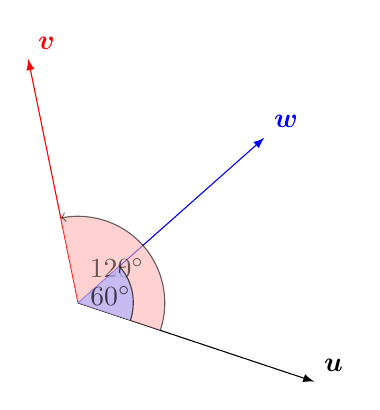
\begin{tikzpicture}[angle radius=1.0cm]
	% \draw[-latex] (0,0)--(3,1);
	\draw[-latex] (0,0) coordinate (A) -- (3,-1) coordinate (B) node[anchor=south west]{$\boldsymbol{u}$};
	\draw[-latex, red] (0,0) to ({atan(-1/3)+120}:{sqrt(10)}) coordinate (C) node[anchor=south west]{$\boldsymbol{v}$};
	\draw[-latex, blue] (0,0) to ({atan(-1/3)+60}:{sqrt(10)}) coordinate (D) node[anchor=south west]{$\boldsymbol{w}$};
	\draw pic ["$120^\circ$", draw, ->, fill=red!30, angle radius=1.1cm,opacity=0.6] {angle = B--A--C};
	\draw pic ["$60^\circ$", draw, ->, fill=blue!30, opacity=0.7, angle radius=0.7cm] {angle = B--A--D};
\end{tikzpicture}

\end{document}
